\documentclass[11pt]{article}
\usepackage{setspace}
\usepackage[a4paper,margin=1in]{geometry}
\geometry{margin=0.85in}
\setstretch{1.0}
\usepackage{graphicx}
\usepackage{array}
\usepackage{setspace}
\usepackage{parskip}
\usepackage{ragged2e}

\pagestyle{empty}
\setstretch{1.05}

\begin{document}


% Title
\begin{center}
    {\Large \textbf{Job Application}} \\[3cm]
    
    {\Huge \textbf{Zhongli Wang}} \\[0.4cm]
    
    {\huge Application for Quantitative Researcher}
\end{center}

\vspace{0.6cm}

% Large picture in the middle
\begin{center}
    \IfFileExists{../zhongli-wang-profile.jpg}{
        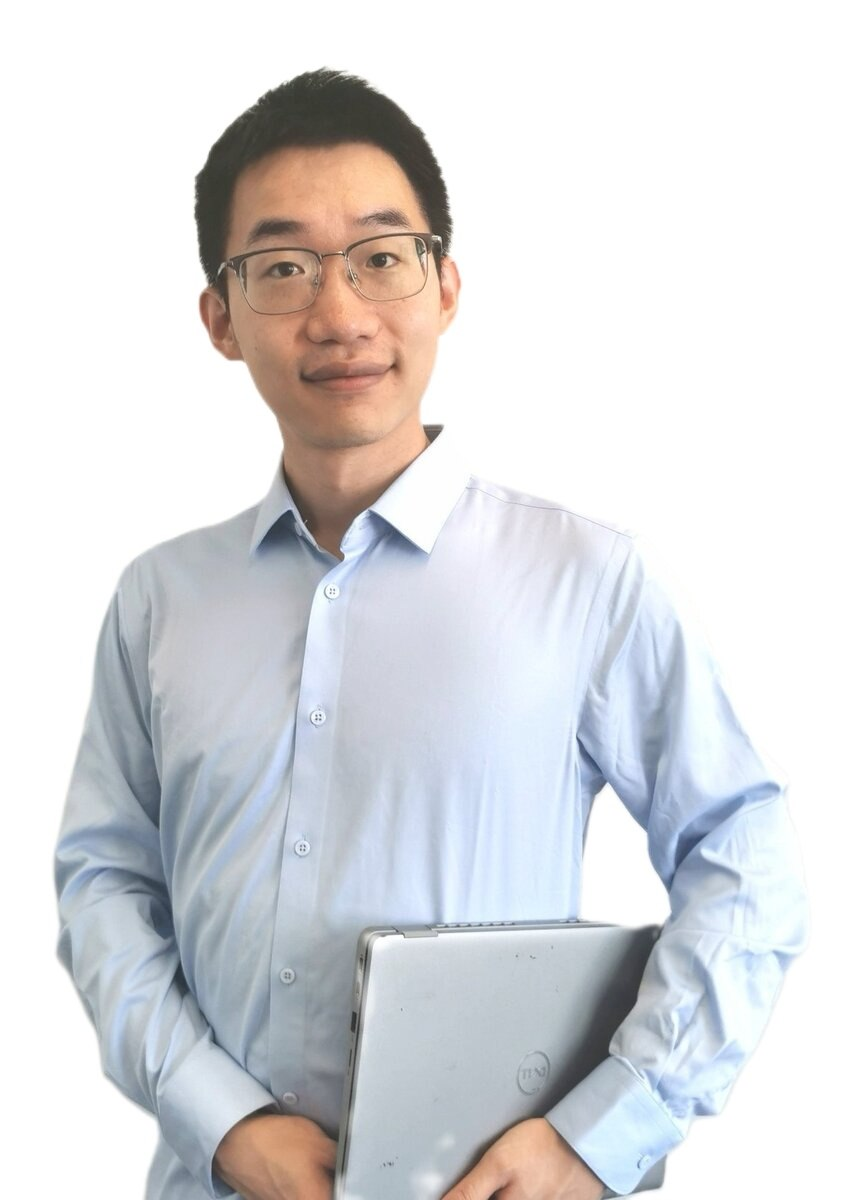
\includegraphics[
            width=0.55\textwidth,
            height=0.45\textheight,
            keepaspectratio
        ]{../zhongli-wang-profile.jpg}
    }{
        \vspace{0.45\textheight}
    }
\end{center}

\vspace{0.7cm}

% \vspace{3cm}


% Personal details
\begin{center}
\renewcommand{\arraystretch}{1.35}
\begin{tabular}{>{\bfseries}p{4.2cm} p{8.5cm}}


Address: & Astastrasse 22, 33617 Bielefeld, Germany \\

Number: & +49 160 9541 6015 \\

Email: & nkwangzhongli@gmail.com \\
\end{tabular}
\end{center}

\vfill

% \begin{center}
%     \small Last updated: \today
% \end{center}
\newpage
\enlargethispage{4\baselineskip}

\begin{flushright}
Zhongli Wang \\
Astastrasse 22 \\
33617 Bielefeld \\
Germany \\
\end{flushright}

\vspace{0.1cm}

\noindent
Anson McCade \\
Hong Kong

\vspace{0.1cm}

\noindent
Application for Quantitative Researcher, Fundamental/Alternative Data \\

\vspace{0.05cm}

\noindent Dear Anson McCade Hiring Team,

I am writing to apply for the Quantitative Researcher, Fundamental/Alternative Data position in Hong Kong. 
I am completing the final stage of my Ph.D. in Economics at Bielefeld University, with my defense scheduled for September 21, 2026, 
and I also hold an M.A. in Business and Economics with a Banking and Finance major and a B.Sc. in Finance. 
My background combines statistical modeling, Python-based computational research, financial data analysis, and machine learning.

The role's focus on cleaning fundamental or alternative datasets, researching factors, and testing models for equity index returns is closely aligned with how I work. 
In my doctoral research, I build computational models, estimate parameters, and test how market structure changes outcomes under uncertainty. 
In a published fraud detection project, I used accounting, financial, and market indicators with XGBoost and LightGBM to identify red flags in listed companies.

I would bring the following strengths to the quantitative research mandate:

\begin{itemize}
    \item \textbf{Fundamental data research:} Experience structuring accounting, financial, and market indicators into model-ready datasets for supervised learning and empirical analysis.
    \item \textbf{Python and R modeling:} Advanced Python skills, plus R, Julia, Mathematica, and SQL foundations for reproducible data processing, estimation, and robustness checks.
    \item \textbf{Backtesting discipline:} Training in econometrics, SMM, MCMC, and model validation, with attention to out-of-sample testing, sensitivity checks, and interpretable results.
    \item \textbf{LLM and workflow tools:} Experience with AutoGen, LangChain, the OpenAI API, Claude Code, Git, LaTeX, and research automation for documented analytical workflows.
\end{itemize}

I am interested in this Hong Kong-based opportunity because it connects my finance training with practical factor research, portfolio analysis, and systematic testing. 
Although my previous work has been research-focused rather than a dedicated hedge-fund seat, the analytical core is directly relevant: preparing noisy datasets, testing predictive signals, validating model behavior, and communicating results clearly.

Thank you for your time and consideration. 
I would welcome the opportunity to discuss how my research background, financial training, and coding experience can contribute to this Quantitative Researcher mandate.

\vspace{0.05cm}
\noindent Sincerely, \\[0.08cm]
\noindent Zhongli Wang \\[-0.2cm]

\vspace{0.1cm}
\noindent
\includegraphics[width=2.7cm,keepaspectratio]{../Wang-sig.jpg}

\end{document}
